\documentclass[12pt]{article}
\usepackage{amsmath}
\usepackage{indentfirst}
\setlength{\parindent}{0em}
\usepackage{graphicx}
\usepackage{setspace}

%粗体字
\newcommand{\bb}[1]{{\textbf {#1}}}
%下划线
\newcommand{\uu}[1]{\underline{#1}}
%求极限
\newcommand{\infinity}{\infty}
%分式求导
\newcommand{\fp}[2]{\frac{\partial{#1}}{\partial{#2}}}
%加总公式
\newcommand{\addup}[4]{\sum\limits_{#1 = #2} ^#3 {#4}}
%连乘公式
\newcommand{\pai}[4]{\prod_{#1 = #2} ^#3 {#4}}
%求极限
\newcommand{\Lim}[3]{\lim_{#1 \to #2} {#3}}
%可调整大小的括号
\newcommand{\bkt}[1]{\left( {#1} \right)}
%积分
\newcommand{\integral}[3]{\int_{#1}^{#2}{#3}}
%行内公式
\newcommand{\e}[1]{$ #1 $}
%行间公式
\newcommand{\ee}[1]{$$ #1 $$}




\title{Notes for Game Theory}
\author{Synferlo}
\date{August 29, 2020}


\begin{document}
\begin{spacing}{1.5}
    \maketitle
    
    \newpage  
    \section{Lecture 1}
        \begin{flushright}
            Date: August 24, 2020    
        \end{flushright}
        

        \subsection{Strategic Interdependent (S.I.)}
            
            {\textbf DEF:}\\ If you know your rival's choices, you could find your best choice.
            And your best choice is vary with your rival's choices.\\

            \bb{Example:}\\ Coke's best choices often depends on Pepsi's choice of pricing,
            ads, new product information, etc.\\

            \bb{S.I.} does not fit with 2 standard approaches:

            \begin{itemize}
                \item Perfect competition: Because Coke affects mkt outcome.
                \item Monopoly: Pepsi also affect mkt outcomes.
            \end{itemize}

            \bb{Some History:}\\ In 1970s, economists got interested in strategic Interdependent.
            Rediscovered work on game theory from 1950s.\\

            \bb{S.I. Application:}

            \begin{itemize}
                \item I.O: pricing, capacity choice, cartel.
                \item Labor: negotiation, strikes, compensation, schemes.
                \item International trade: strategic trade policy.
                \item Macro: money supply/inflation.
                \item Law and Econ: Jury rules, settling law suit, allocation court costs.
                \item Political: International relations.
                \item Biology: competition for food and shelter.
                \item Industrial Engineering: autonomous vehicles.
            \end{itemize}

            \bb{Important Point:}\\ Game theory is just an extension of basic 801, i.e.
            individual decision making. Payoff-maximizer interacting with other payoff maximizer,
            in setting strategic interdependence.
        
        \subsection{Chuck's Approach for This Course.}

            \bb{Part I:}\\ Introduce concepts/tools, which is very abstract and almost no economics.
            Then, we goes to four types of games and their associated equilibrium concepts.
            
            \begin{center}
                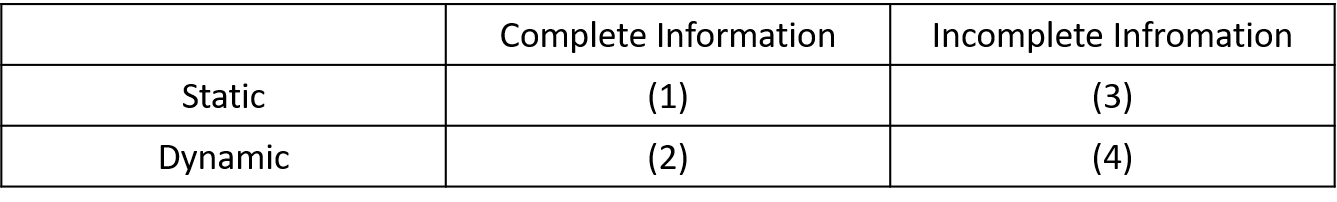
\includegraphics[scale = 0.5]{pic/lecture1/four_types_games.png}
            \end{center}

            \bb{Part II:} Standard game-theoretic models
            
            \begin{itemize}
                \item Models that all economists should know.
                \item Tips/tricks/techniques for solving broad classes of model.
            \end{itemize}

            \bb{Part III:} Information Economics

            \bb{Part IV:} Auctions and Mechanism Design\\

    \newpage
    \section{Lecture 2}
        \begin{flushright}
            Date: August 26, 2020    
        \end{flushright}
        

        \subsection{Game Theory Basics}

            When formalize a strategic scenario, think about relevant structural features:

            \begin{itemize}
                \item Who are the players?
                \item What can they do?
                \item What are payoffs for different combinations of choices by all players?
                \item What is timing of moves?
                \item What information is available to players at every point in time?
            \end{itemize}

            Let's start with static games of complete Information:
            
            \begin{itemize}
                \item All players make simultaneous choices, once (one-time decision making).
                \item All players have \underline{common knowledge (C.K.)} about 
                      game's structure: players, payoffs, timing, information, etc.
            \end{itemize}

            NB: C.K. refers to every player know everything about the game.\\

            Now, let's be formal:
            \begin{itemize}
                \item \bb{Players}: Normally indexed by \e{i, i = 1,2,3,...,N}.
                \item \bb{Strategies}:\e{S_i} is a set of strategies available to player \e{i}.
                                        it could be infinite/finite, and encompass dynamics 
                                        (NOT in static games).
                \item \bb{Payoffs}: \e{u_i: \times_{j = 1}^N S_j \rightarrow \bb{R}}, player \e{i}'s payoff is a function
                                    of all player's strategies.
            \end{itemize}
           
                \subsubsection{Strategic-form game}
                    Define a strategic form game as
                    \ee{G = (S_i, u_i)_{i = 1}^N}
                    
                    Notice: \e{\times_{j = 1}^N S_j} is the cross product of all \e{s_j}\\

                    Consider
                    \ee{S = \times_{j = 1}^N S_j \quad s \in S,}
                    then we can write \e{s = (s_1,s_2,...,s_N)}.\\

                    Each \e{S_j} is a vector (each element of S), where a particular vector is the strategies for
                    particular player.

                    \bb{Example:}\\

                    Now, let's try to formalize the half-average game we have played on Monday. The game requires each
                    player say a number from 1 to 100. The closest number to the half-average (\e{HA = \frac{Ave}{2}})
                    get \$5 reward.\\

                    \bb{(1)Strategy space:}\\
                    \ee{S_i = \{ 1,2,...,100\}}
                    Or 
                    \ee{S_i = \{x| x \in \{1,2,...,100\}\} }

                    \bb{(2)Payoffs:}

                    
                    \begin{align*}
                        u_i &=
                        \begin{cases}
                            \emptyset \quad & if |s_i - HA| > \min_j |s_j - HA|\\
                            \frac{5}{|w|} \quad & if |s_i - HA| = \min_j |s_j - HA|
                        \end{cases}\\[5pt]
                        HA & = \frac{\addup{j}{1}{n}{s_j}}{2N}\\[5pt]
                        w & = \{k:|s_k - HA| = \min_j |s_j - HA|\}
                    \end{align*}

                    
                    \begin{itemize}
                        \item \e{|s_i - HA|} refers to the distance of your answer and HA
                        \item \e{\min_j |s_j - HA|} is the nearest distance to HA, which is the distance can win the game.
                        \item k refers to how many players win the game. k can be greater than 1 when multiply player have same distance.
                        \item w is the set of winners. \e{|w|} is not the \bb{absolute value}. It is the number of winners.
                    \end{itemize}
                    

        \subsection{Dominant Strategy}

            \subsubsection{Intuition}

                Consider players R and C in a one-shot, simultaneous-move game. Each player has 2 choices:
                \e{\{R_1, R_2\}, \{C_1, C_2\}}.
                Payoffs are \e{\{ \pi_R, \pi_C\}} for different combination of actions as following:
                \begin{center}
                    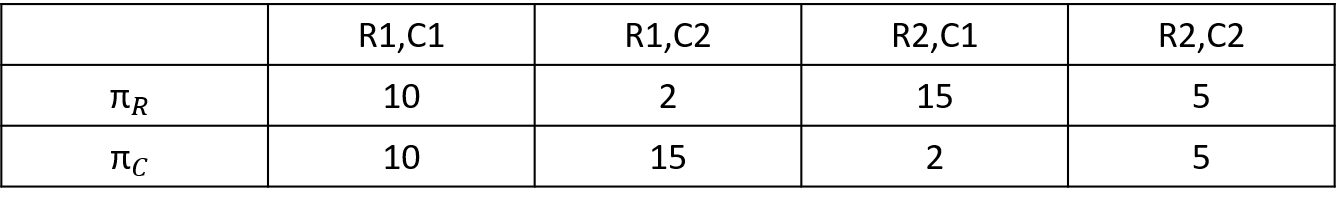
\includegraphics[scale = .5]{pic/lecture2/basic_prisoner_initial.png}
                \end{center}

                How do you think the player will choose?
                Let's write down the payoff matrix in this way.

                \begin{center}
                    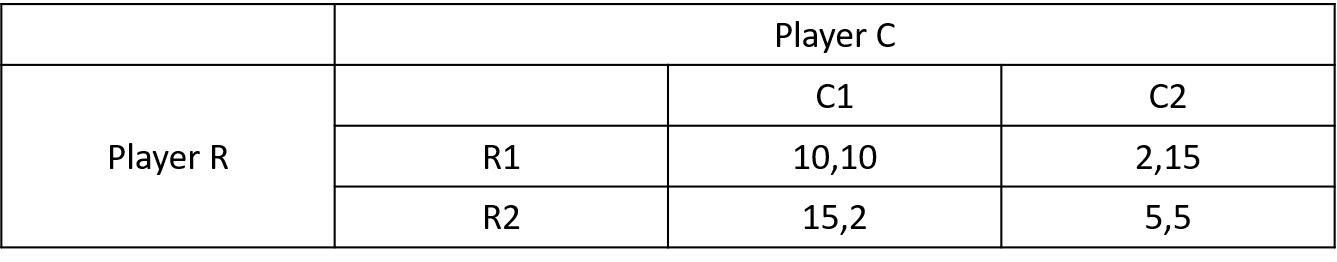
\includegraphics[scale = .5]{pic/lecture2/basic_prisoner_dilemma.png}
                \end{center}

                If you are player R, think about payoffs from different combinations of strategies.

                \begin{itemize}
                    \item If C chooses \e{C_1}, then R prefers \e{R_2}, because \e{15 > 10}.
                    \item If C chooses \e{C_2}, then R prefers \e{R_2}, because \e{5 > 2}.
                \end{itemize}
            
                So, whatever C choose, R will choose \e{R_2}. Then, we call \e{R_2} is a \bb{\underline{dominant strategy}}
                that maximizes player's payoff, \underline{regardless} of rival's choice.\\

            \subsubsection{Formalization}

                Now, let's be formal:\\

                (1) For all players' strategies:
                \ee{ S = \times_(j = 1)^N S_j}
                \ee{ s \in S, \quad s_i = (s_1,s_2,...,s_N)}

                (2) For all players' strategies without player \e{i}'s:
                \ee{ S_{-i} = \times_{j \neq i} ^N S_j}
                \ee{ s_{-i} \in S_{-i}, \quad s_{-i} = (s_1,s_2,...,s_{i-1},s_{i+1},...,s_N)}

                \bb{NB:} we define \e{-i} as all players except player \e{i}. So, \e{S_{-i}} is the joint
                strategy space except player \e{i}.\\

                \bb{Definition:}
                A strategy \e{\hat{s_i}} for player \e{i} is \bb{\underline{strictly dominat}} If
                \ee{u_i(\hat{s_i}, s_{-i}) > u_i(s_i, s_{-i}) \quad \forall s_{-i} \in S_{-i}, s_i \neq \hat{s_i}}
                
                Notice, \e{u_i(\hat{s_i},s_{-i})} means the payoff you will receive if you choose \e{\hat{s_i}}, and
                other player choose \e{s_{-i}}.\\
                So, \e{\hat{s_i}} is dominant strategy if the payoff choosing it is greater than all other strategies
                you will choose, no matter what strategy is chosen by others.\\
                We can have \bb{\underline{weakly dominant}} if replace "\e{>}" with "\e{\ge}", i.e.
                \ee{u_i(\hat{s_i}, s_{-i}) \ge u_i(s_i, s_{-i})}.
            
        \subsection{Dominate and Dominated}

            Now let's view \bb{dominant strategy} from another perspective:\\
            \e{R_1} is worse than \e{R_2}, no matter what C does. Then, we say that \e{R_1} is 
            a \bb{\underline{dominated strategy}}. It is dominated by \e{R_2}.\\
            
            \bb{Definition:}\\
            Player \e{i}'s strategy \e{\bar{s_i}} is \bb{strictly dominated} if \e{\exists \tilde{s_i}}
            \ee{u_i(\tilde{s_i}, s_{-i}) > u_i(\bar{s_i}, s_{-i}) \quad \forall s_{-i} \in S_{-i}}.

            \bb{Alternative:}\\
            Player \e{i}'s strategy \e{\tilde{s_i}} \bb{strictly dominates} another strategy \e{\bar{s_i}} if:
            \ee{u_i(\tilde{s_i}, s_{-i}) > u_i(\bar{s_i}, s_{-i}) \quad \forall s_{-i} \in S_{-i}}
            we can also define "\bb{weakly dominate}" by replacing "\e{>}" with "\e{\ge}".\\

            Games with this structure is referred to as \underline{Prisoner's Dilemma}.
            \begin{itemize}
                \item US vs Russia (arms races)
                \item Advertisement
                \item Pricing
                \item Hiring lawyer
                \item ...

            \end{itemize}

    \newpage
    \section{Lecture 3}
        \begin{flushright}
            Date: August 28, 2020    
        \end{flushright}
        

        \subsection{Iterated Elimination}
            $$$$
            How to play this game?

            \begin{center}
                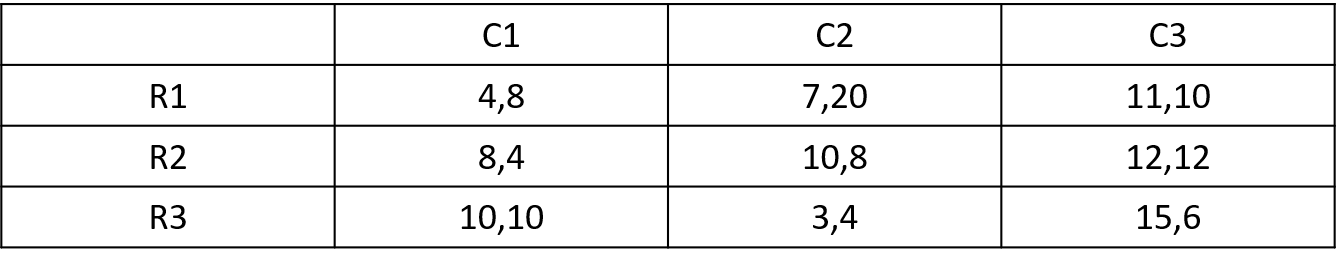
\includegraphics[scale = .5]{pic/lecture3/iterated_elimination_initial.png}
            \end{center}
            
            Obviously, there is NO dominant strategy for each player. But for player R, \uu{\e{R_2}
            is always better than \e{R_1}}, whatever C does.\\
            So, R will never choose \e{R_1}. \e{R_1} is ruled out! The game becomes this:

            \begin{center}
                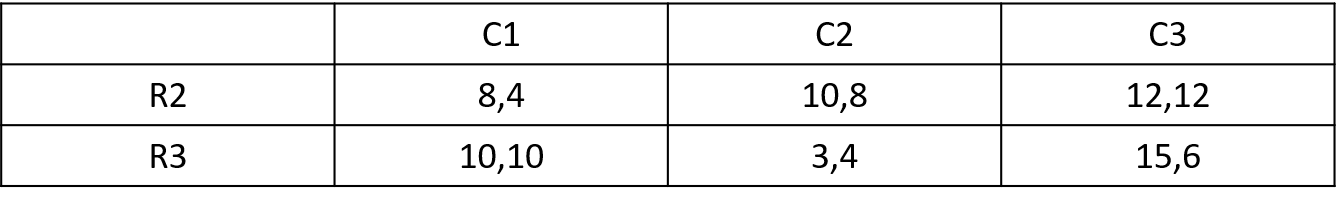
\includegraphics[scale = .5]{pic/lecture3/IE_R1_rule_out.png}
            \end{center}

            We say \e{R_2} is strictly better than \e{R_1}, or \underline{\e{R_2} strictly
            dominates \e{R_1}.}\\
            Then, in the revised game, we see, for player C, \underline{\e{C_3} strictly
            dominates \e{C_2} \e{(12 > 8, 6 > 4)}}.\\
            So, C will never choose \e{C_2}.\\

            Then, the game looks like this:

            \begin{center}
                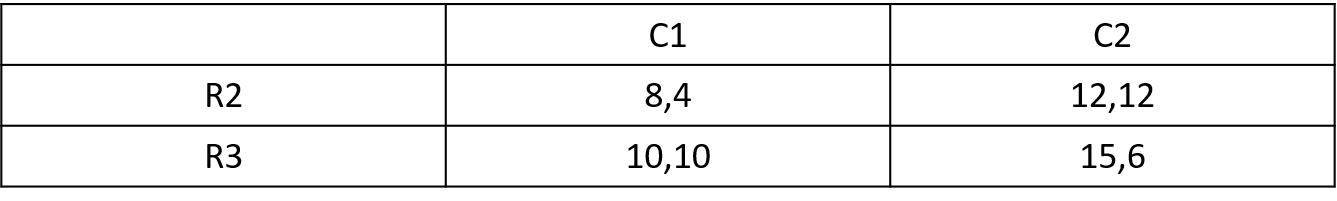
\includegraphics[scale = .5]{pic/lecture3/IE_R1_C2_rule_out.png}
            \end{center}

            For player R, \underline{\e{R_3} strictly dominates \e{R_2 (10 > 8, 15 >12)}}.
            Then, if C know R will pick up \e{R_3}, C will choose \e{C_1, (10 > 6)}.\\
            So, game ends up with \e{(R_3, C_1) \rightarrow (10,10)}.\\

            The main idea of this game is to find the strategies can strictly dominates others.
            The process of \uu{iterated elimination of strictly dominated strategies}, is called
            IESDS.\\
            Or called:\\
            (1) IEWDS: Iterated elimination of weakly dominated strategies.\\
            (2) IEDS: Iterated elimination of dominated strategies.\\

            So, IEDS can eliminate some strategies from consideration as equilibrium.
            And it might  get to unique prediction.\\

            Now, let's reconsider the half-average game. A rational player will never choose
            number that is above 50. Why? Even if everyone choose 100, the
            \e{HA = \frac{\sum100}{n} \times \frac{1}{2} = 50}, so \e{HA_0 \in [0,50]}.
            With this consideration, if everyone know \e{HA_0 \in [0,50]}, rational players will not
            choose number above 25, as \e{HA_1 \in [0,25]}. Then, players will not choose number above
            12.5, ..., and so forth.
            In the end, everyone will choose 1.

        \subsection{Best Response (BR)}

            Now consider a new game.
            
            \begin{center}
                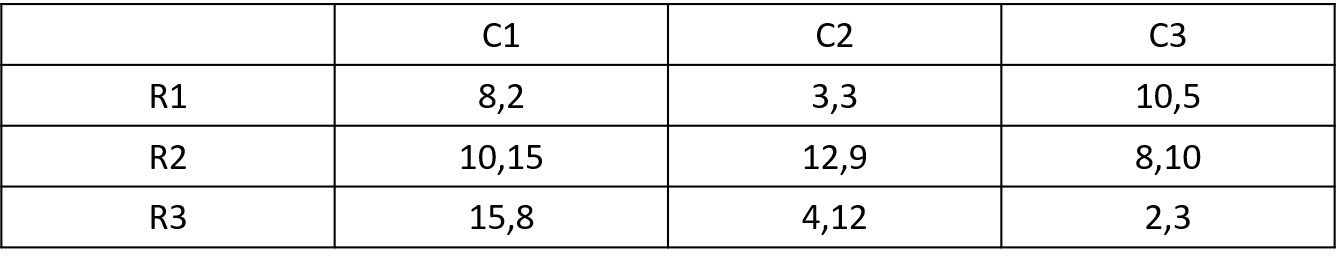
\includegraphics[scale = .5]{pic/lecture3/best_response_game_initial.png}
            \end{center}

            In this game, IEDS does nothing because there is NO strategy can be strictly
            dominated by the others. Let's think about the \uu{Best Responses (BRs)}.
            \bb{DEF:} BR is payoff maximizing choice for a particular choice chose by rival.\\
            
            (1) For player R:

            When C chooses \e{C_1}, \e{R_3} is the best. \e{ \{ R_3, C_1 \}}.\\
            When C chooses \e{C_2}, \e{R_2} is the best. \e{ \{ R_2, C_2 \}}.\\
            When C chooses \e{C_3}, \e{R_1} is the best. \e{ \{ R_1, C_3 \}}.\\

            (2) For player C:

            When R chooses \e{R_1}, \e{C_3} is the best. \e{ \{ R_1, C_3 \}}.\\
            When R chooses \e{R_2}, \e{C_1} is the best. \e{ \{ R_2, C_1 \}}.\\
            When R chooses \e{R_3}, \e{C_2} is the best. \e{ \{ R_3, C_2 \}}.\\

            \begin{center}
                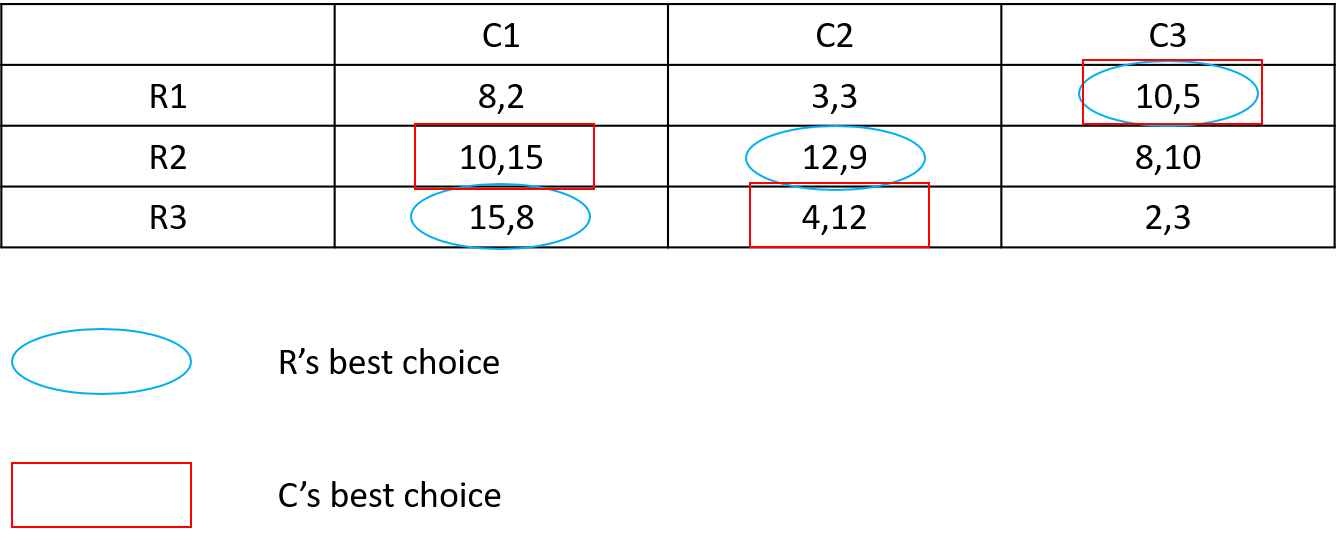
\includegraphics[scale = .5]{pic/lecture3/BR_circled.png}
            \end{center}

            Clearly \e{ \{R_1, C_3 \}} is the only one choice that is selected by both players.
            \e{ \{R_1, C_3 \}} is the only combination of strategies for which each player 
            is \uu{best-responding} to rival's choice.

        \subsection{Nash Equilibrium (N.E.)}

            \bb{Informal Definition:}\\
            A set of strategies, one for each player, that are \uu{mutual best-responses}.

            \bb{Formal Definition:}\\
            For a strategic-form game \e{G = (S_i, u_i)_{i = 1}^N} that joint strategy
            \e{\hat{s} \in S} is a \uu{pure strategy nash equilibrium} if for all \e{i}:
            \ee{u_i(\hat{s_i}, \hat{s_{-i}}) \ge u_i(s_i, \hat{s_{-i}}) \quad \forall s_i \in S_i} 

            \e{u_i(\hat{s_i}, \hat{s_{-i}})} is the payoff that all players choose \e{\hat{s}} type
            of strategy.\\
            \e{u_i(s_i, \hat{s_{-i}})} is the payoff that all other players choose \e{\hat{s}} 
            but you DO NOT.

            \bb{Important:}\\
            \e{\hat{s_i}} is a best-response to \e{\hat{s_{-i}}}. But it is not necessarily a 
            best-response to \uu{any} (or every) \e{s_{-i}}. \\

            N.E. is the strategies, not the payoffs. So, in our game, N.E. is
            \e{ \{R_1, C_3 \}}. BR illustrates link between \uu{game theory and decision theory}
            (or 'monopoly' theory). BR is 'monopoly choice: holding rival's choice constant,
            \begin{quotation}
                It means we hold \e{C_1} and find best \e{R_i}, then hold \e{C_2} and find best \e{R_i}...
            \end{quotation}

            N.E. is the intersection of BR function.\\

            Then questions come up:
            \begin{enumerate}
                \item Does games tend to have N.E. ?
                \item Can a game have multiple N.E. ?
            \end{enumerate}

            For the first question, the answer is YES, if we modify one thing.\\
            For the second question, the answer is YES. we can even have a game with \uu{infinite}
            numbers of N.E. But if so, we cannot predict how players are going to make decision.\\

            Good exercise for constant \e{3 \times 3} games such that:
            \begin{enumerate}
                \item No dominant strategy but IEDS gives unique solution.
                \item IEDS does nothing but intersecting BR function does.
                \item No mutual BRs(BR function do not intersect)
            \end{enumerate}

            To ensure existence of N.E., we need to \uu{enrich the strategy space}.
            Consider a game like this:

            \begin{center}
                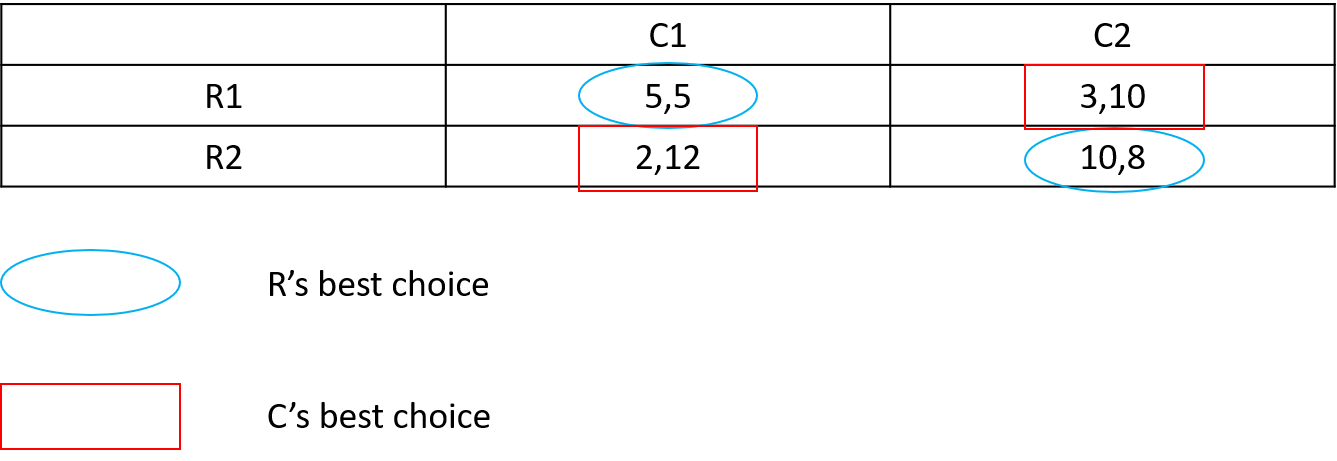
\includegraphics[scale = .5]{pic/lecture3/game_need_prob.png}
            \end{center}

            There is no intersecting BRs. Now what? How to \uu{enrich the strategy space?}\\
            Answer: we need to let the strategies include a random component(Prob.).
            Strategies considered so far, in our class, are \uu{pure strategies}(P.E.).
            P.E. means the particular choice is made with \e{Prob. = 1}. Now, we are going
            to design a \uu{mix strategy}, puts Prob. mass on one or more P.E.\\
            For example:\\
            Play \e{R_1} with \e{Prob. = .3}\\
            Play \e{R_2} with \e{Prob. = .7}

            We will discuss this next week!
            


            
            
\end{spacing}
\end{document}
